\documentclass[12pt,fleqn]{article}\usepackage{../common}
\begin{document}
Gaussian Karisimlari ile Deri Rengi Saptamak

Bir projemizde dijital resimlerdeki deri rengi iceren kisimlari cikartmamiz
gerekiyordu; cunku fotografin diger renkleri ile ilgileniyorduk (resimdeki
kisinin uzerindeki kiyafetin renkleri) ve bu sebeple deri renklerini ve o
bolgeleri resimde saptamak gerekti. Bizim de onceden aklimizda kalan bir
tembih vardi, Columbia Universitesi'nde yapay ogrenim dersi veren Tony
Jebara derste paylasmisti bir kere (bu tur gayri resmi, lakirdi seviyesinde
tiyolar bazen cok faydali olur), deri rengi bulmak icin bir projesinde tum
deri renklerini R,G,B olarak grafige basmislar, ve beyaz olsun, zenci
olsun, ve sonuc grafikte deri renklerinin cok ince bir bolgede yanyana
durdugunu gormusler. Ilginc degil mi?

Buradan su sonuc cikiyor ki diger renklerin arasinda deri renklerine
odaklanan, onlari ``taniyan'' bir yapay ogrenim algoritmasinin oldukca
sansi vardir. Ama ondan once veriye bakip grafiksel olarak ne oldugunu
gorelim. 

\begin{minted}[fontsize=\footnotesize]{python}
import pandas as pd, zipfile
with zipfile.ZipFile('skin.zip', 'r') as z:
    d =  pd.read_csv(z.open('skin.csv'),sep=',')
print d[:3]
\end{minted}

\begin{verbatim}
   Unnamed: 0   rgbhex   skin         r         g         b         h  \
0           0  #200e08  False  0.125490  0.054902  0.031373  0.041667   
1           1  #6d6565  False  0.427451  0.396078  0.396078  0.000000   
2           2  #1f2c4d  False  0.121569  0.172549  0.301961  0.619565   

          s         v  
0  0.750000  0.125490  
1  0.073394  0.427451  
2  0.597403  0.301961  
\end{verbatim}

Burada onemli olan R,G,B ve H,S,V kolonlari. Bu iki grup degisik renk
kodlama yontemini temsil ediyorlar. Grafikleyelim,

\begin{minted}[fontsize=\footnotesize]{python}
nd = d[d['skin'] == False]
sd = d[d['skin'] == True]
plt.plot(nd['r'],nd['g'],'.')
plt.hold(True)
plt.plot(sd['r'],sd['g'],'rx')
plt.savefig('stat_gmm_01.png')
\end{minted}


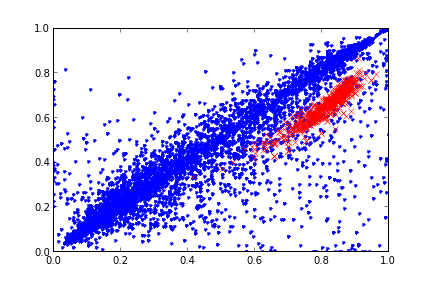
\includegraphics[height=6cm]{stat_gmm_01.png}


















\end{document}
